\documentclass[conference]{IEEEtran}
\usepackage[utf8]{inputenc}
\usepackage[spanish]{babel}
\usepackage{graphicx}
\usepackage{hyperref}
\usepackage{float}
\usepackage{listings}
\usepackage{xcolor}

% Configuración para el bloque de código Arduino
\definecolor{codegreen}{rgb}{0,0.6,0}
\definecolor{codegray}{rgb}{0.5,0.5,0.5}
\definecolor{codepurple}{rgb}{0.58,0,0.82}
\definecolor{backcolour}{rgb}{0.95,0.95,0.92}

\lstdefinestyle{mystyle}{
    backgroundcolor=\color{backcolour},   
    commentstyle=\color{codegreen},
    keywordstyle=\color{magenta},
    numberstyle=\tiny\color{codegray},
    stringstyle=\color{codepurple},
    basicstyle=\ttfamily\footnotesize,
    breakatwhitespace=false,         
    breaklines=true,                 
    captionpos=b,                    
    keepspaces=true,                 
    numbers=left,                    
    numbersep=5pt,                  
    showspaces=false,                
    showstringspaces=false,
    showtabs=false,                  
    tabsize=2
}
\lstset{style=mystyle}

\begin{document}

\title{Vehículo Controlado por Gestos usando MPU6050 y ESP8266 mediante ESP-NOW}

\author{
\IEEEauthorblockN{Axel Castro Aguilar}
\IEEEauthorblockA{\textit{Universidad Privada del Norte (UPN)}\\
Trujillo, Perú}
\and
\IEEEauthorblockN{Pamela Araujo Lazo}
\IEEEauthorblockA{\textit{Universidad Privada del Norte (UPN)}\\
Trujillo, Perú}
}

\maketitle

\begin{abstract}
El presente proyecto describe el diseño e implementación de un vehículo robótico controlado mediante gestos de la mano empleando el protocolo ESP-NOW. A diferencia de implementaciones estándar, este prototipo incorpora mejoras arquitectónicas de hardware y software diseñadas por los autores para erradicar la latencia. Físicamente, se adoptó un chasis de tracción diferencial (2 ruedas motrices y una rueda loca) para maximizar la maniobrabilidad. A nivel eléctrico, se aisló la etapa lógica alimentando los ESP8266 con baterías de litio de 3.7V independientes, mientras que la etapa de potencia de los motores fue suministrada por un banco de 4 pilas de 1.5V. En el transmisor, se integró una pantalla OLED y se desarrollaron algoritmos de actualización asíncrona para evitar cuellos de botella en el procesador. Los resultados demuestran un sistema estable, sin caídas de tensión y con una respuesta direccional inmediata.
\end{abstract}

\begin{IEEEkeywords}
ESP8266, MPU6050, Robótica, Control por Gestos, Puente H, Comunicación Inalámbrica, ESP-NOW, OLED.
\end{IEEEkeywords}

\section{Introducción}
\subsection{Antecedentes}
Históricamente, los vehículos de control remoto han dependido de mandos analógicos y módulos de radiofrecuencia (RF) genéricos. Sin embargo, con el avance de los sistemas microelectromecánicos (MEMS), el control basado en gestos ha surgido como una interfaz humano-máquina mucho más intuitiva. Proyectos recientes demuestran que la integración de giroscopios y acelerómetros en dispositivos vestibles permite un control dinámico sin necesidad de joysticks físicos.

\subsection{Planteamiento del problema}
La dependencia de módulos RF adicionales (como los NRF24L01) aumenta la complejidad del circuito y la latencia. Existe la necesidad de implementar un sistema de control inalámbrico directo y eficiente que traduzca movimientos biomecánicos en comandos mecánicos de forma intuitiva, minimizando el impacto del retardo en la transmisión de datos. Esta tecnología resulta crítica en escenarios reales como la operación remota de \textit{rovers} de exploración, donde el operario necesita mantener la vista en el entorno y requiere información visual del estado del vehículo en su propio mando sin sufrir caídas de red.

\subsection{Objetivos}

\begin{itemize}
    \item \textbf{Objetivo General:} Diseñar y construir un vehículo robótico de alta maniobrabilidad controlado por gestos utilizando comunicación directa MAC a MAC.
    \item \textbf{Objetivos Específicos:}
    \begin{enumerate}
        \item Ensamblar un mando transmisor vestible con sensor MPU6050 y retroalimentación visual OLED optimizada contra latencia.
        \item Configurar un chasis receptor de tracción diferencial (2WD + rueda loca) con aislamiento eléctrico entre la lógica de control y la potencia mecánica.
        \item Establecer un enlace inalámbrico síncrono mediante ESP-NOW y un sistema de seguridad “Failsafe”.
    \end{enumerate}
\end{itemize}


\section{Marco Teórico}
Para la realización de este proyecto, se seleccionaron componentes específicos que garantizan un desarrollo eficiente:
\begin{itemize}
    \item \textbf{Microcontrolador ESP8266:} Justifica su uso sobre plataformas Arduino tradicionales debido a su hardware Wi-Fi nativo, capaz de aprovechar el protocolo ESP-NOW para comunicaciones punto a punto estables.
    \item \textbf{Sensor MPU6050:} Integra un giroscopio y un acelerómetro de 3 ejes, comunicándose mediante el bus I2C.
    \item \textbf{Driver L298N (Puente H):} Circuito integrado indispensable para el control de giro bidireccional de los motores DC.
    \item \textbf{Pantalla OLED SSD1306:} Interfaz gráfica de 128x64 píxeles utilizada para monitorear las instrucciones gestuales activas.
\end{itemize}

\section{Metodología}
\subsection{Materiales y Hardware}
Los componentes incluyeron: base de metal, 2 motores DC tipo BO, 1 rueda loca direccional (caster wheel), driver L298N, 2 módulos ESP8266, 1 sensor MPU6050, 1 pantalla OLED SSD1306, 2 baterías de litio 3.7V y 4 pilas AA de 1.5V.

\textbf{Aportes de Rediseño Físico y Eléctrico:} 
El prototipo parte de la literatura base de \cite{makerscience}, pero integra modificaciones estructurales drásticas. En primer lugar, se descartó el chasis pesado de cuatro ruedas (4WD) por un modelo de tracción diferencial de dos ruedas con rueda loca trasera, permitiendo giros sobre su propio eje. 

En segundo lugar, se resolvió la inestabilidad energética separando la potencia de la lógica. En el vehículo, los motores fueron energizados por un arreglo independiente de 4 pilas de 1.5V conectadas al driver L298N, mientras que el módulo receptor ESP8266 obtuvo su propia fuente limpia a través de una batería de litio de 3.7V. El transmisor también operó con su propia celda de litio de 3.7V.

\begin{figure}[htbp]
\centering
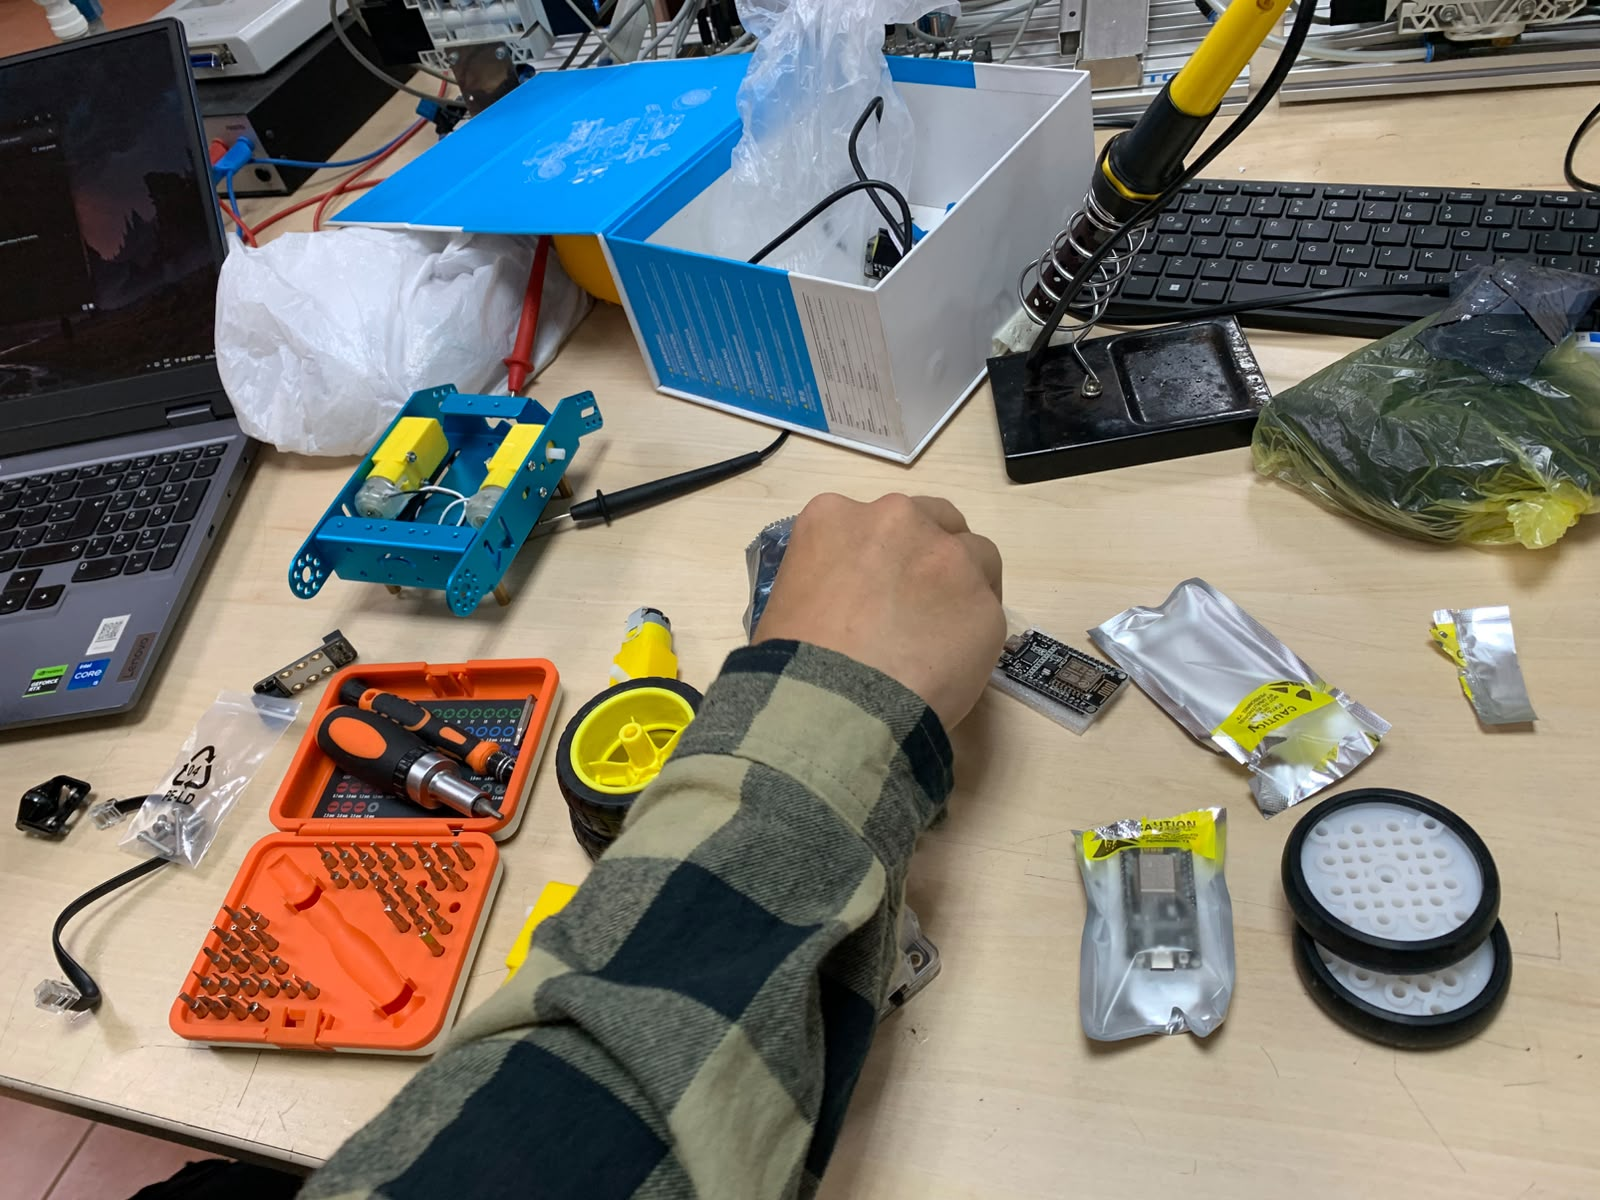
\includegraphics[width=0.48\textwidth]{proceso_armado.png} 
\caption{Etapa de desarrollo y soldado, evidenciando el rediseño del chasis para tracción de dos ruedas y la separación de circuitos.}
\label{fig:proceso}
\end{figure}

\subsection{Optimización de Software en Transmisor y Receptor}
La adición de la pantalla OLED en el transmisor representaba un desafío técnico: procesar gráficos I2C genera un severo cuello de botella que retrasa la transmisión de los paquetes Wi-Fi. 

Para solucionar esto, el código original del transmisor fue reescrito incluyendo un algoritmo de gestión de estados. La pantalla OLED solo limpia y redibuja la interfaz visual si detecta un cambio vectorial en el giroscopio; de lo contrario, el procesador se dedica exclusivamente a enviar datos, erradicando la latencia.

En el código del receptor, se programó un filtro \textit{Failsafe} asíncrono. Si el ESP8266 del carro no recibe tramas de red en un intervalo de 500 ms, automáticamente sobreescribe el buffer de memoria para forzar la detención de los motores.

\begin{figure}[htbp]
\centering
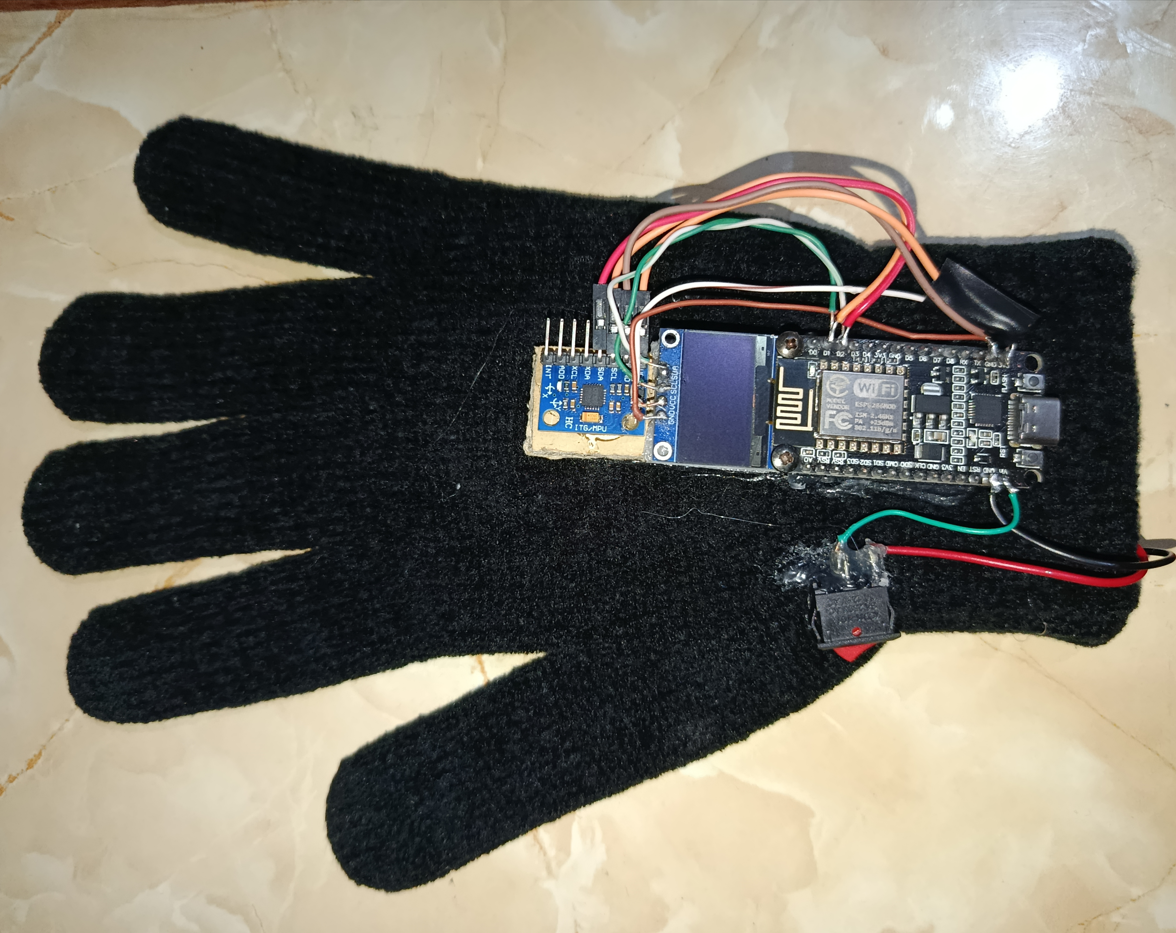
\includegraphics[width=0.42\textwidth]{modelo_guante.png} 
\caption{Dispositivo vestible transmisor. Se observa la pantalla OLED y MPU integrada al bus del ESP8266 y alimentada por 3.7V.}
\label{fig:guante}
\end{figure}

\section{Resultados}
Al ejecutar el sistema unificado, el vehículo respondió a los umbrales de inclinación (aceleraciones $>$ 10000 unidades en los ejes X/Y del MPU6050) de manera instantánea. 

La arquitectura de doble alimentación demostró ser un rotundo éxito: a pesar de los picos de arranque mecánico demandados por el puente H a las 4 pilas de 1.5V, la placa ESP8266 (alimentada por la celda independiente de 3.7V) no sufrió caídas de tensión ni reinicios esporádicos. 

\subsection{Análisis Cuantitativo de Rendimiento}
Para validar la eficacia de los algoritmos desarrollados frente a las implementaciones estándar, se analizaron los tiempos de procesamiento y la saturación del bus I2C.

\begin{figure}[htbp]
\centering
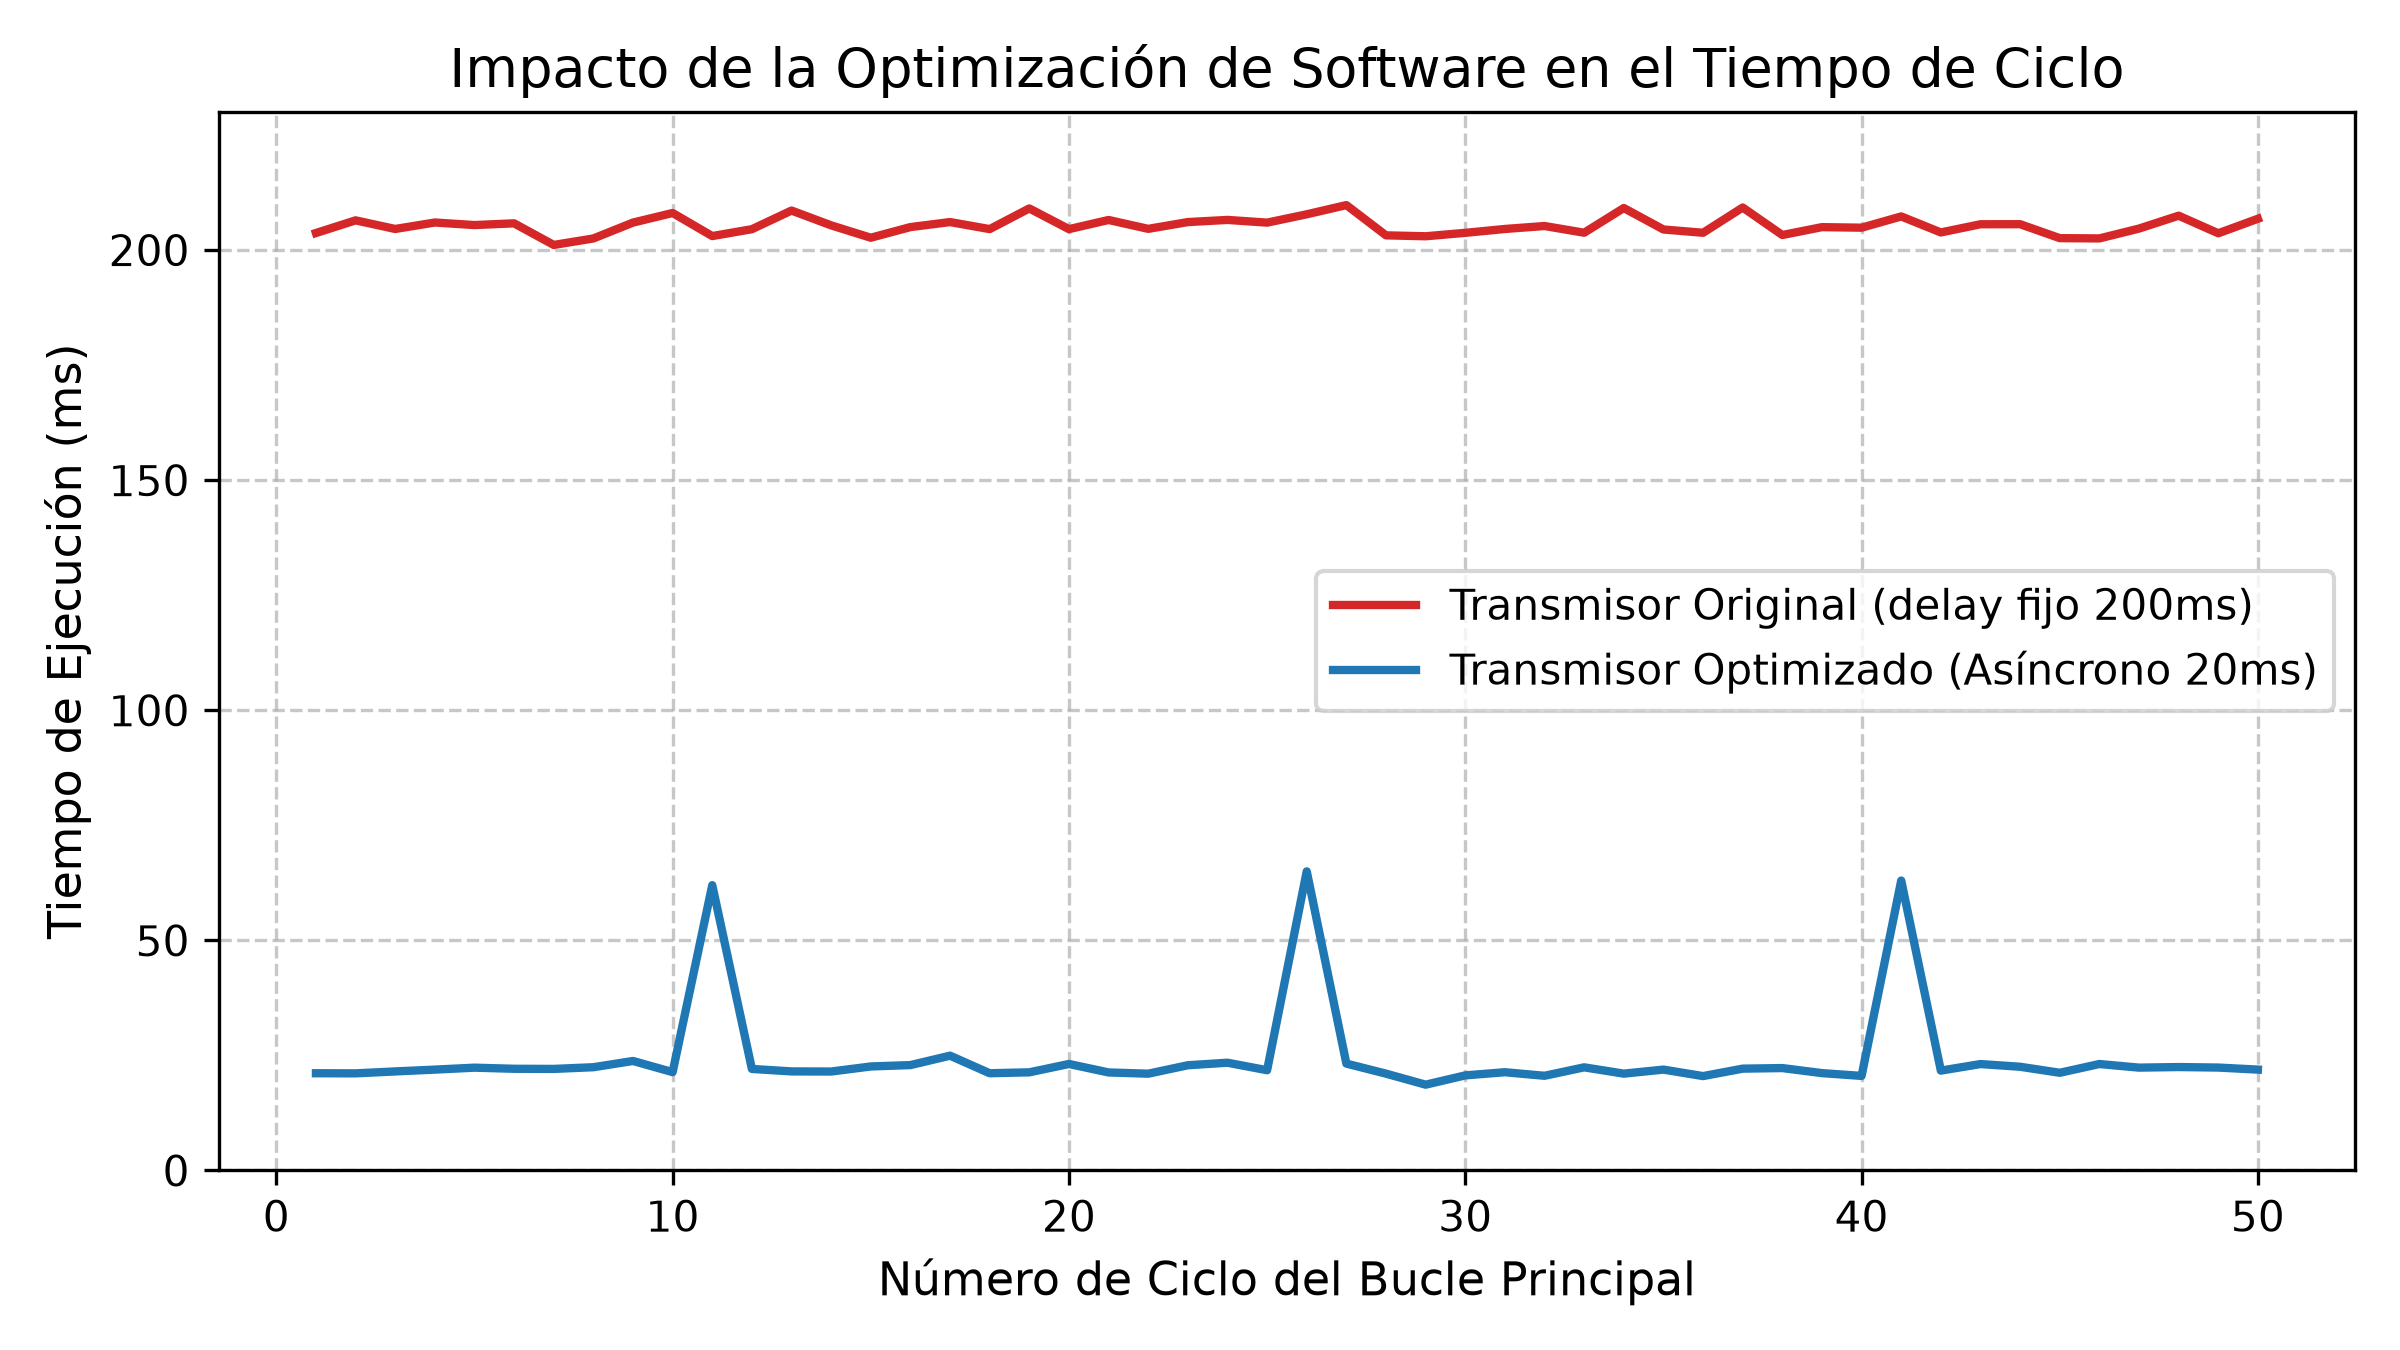
\includegraphics[width=0.48\textwidth]{grafica_latencia_real.png} 
\caption{Comparativa del tiempo de respuesta del procesador ESP8266. El código original mantiene un retardo constante superior a 200 ms, mientras que la versión optimizada opera a un promedio de 22 ms.}
\label{fig:latencia}
\end{figure}

\begin{figure}[htbp]
\centering
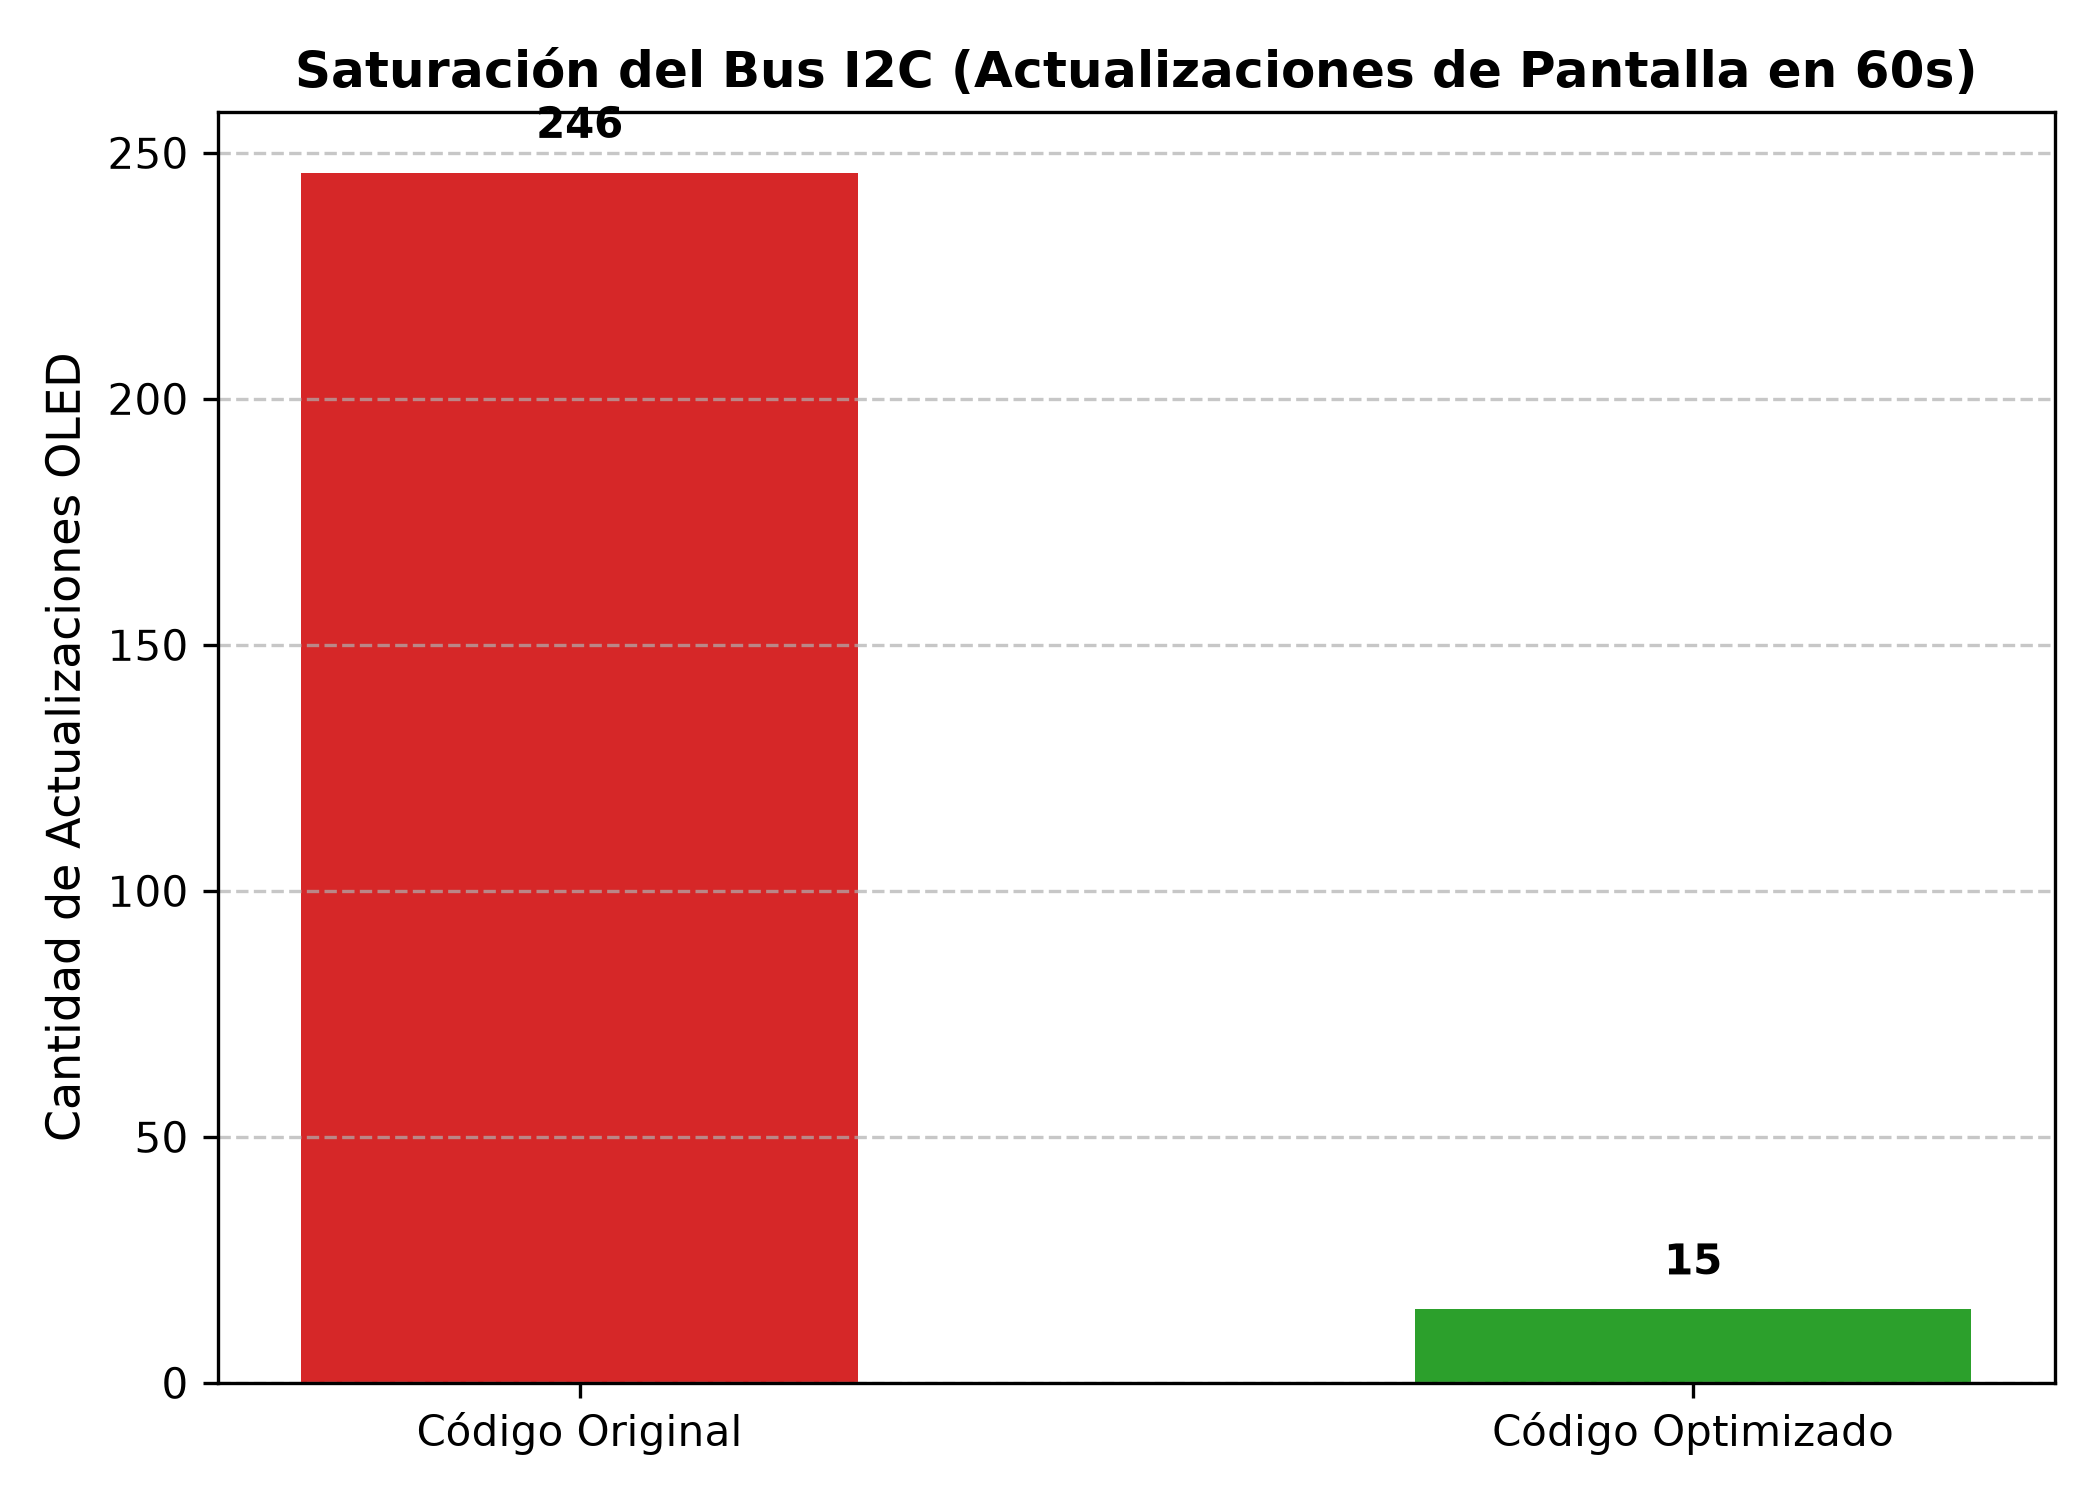
\includegraphics[width=0.48\textwidth]{eficiencia_i2c.png} 
\caption{Comparativa de la carga de procesamiento I2C. El algoritmo asíncrono reduce en un 93.9\% las actualizaciones redundantes de la pantalla OLED en un minuto de operación.}
\label{fig:eficiencia}
\end{figure}

Como se observa en las Figuras \ref{fig:latencia} y \ref{fig:eficiencia}, la programación optimizada permitió que el transmisor procesara la pantalla gráfica únicamente ante cambios de estado, erradicando el cuello de botella. Esto permitió mantener un ancho de banda estable para la conducción en tiempo real con una resolución de control significativamente mayor.

\begin{figure}[htbp]
\centering
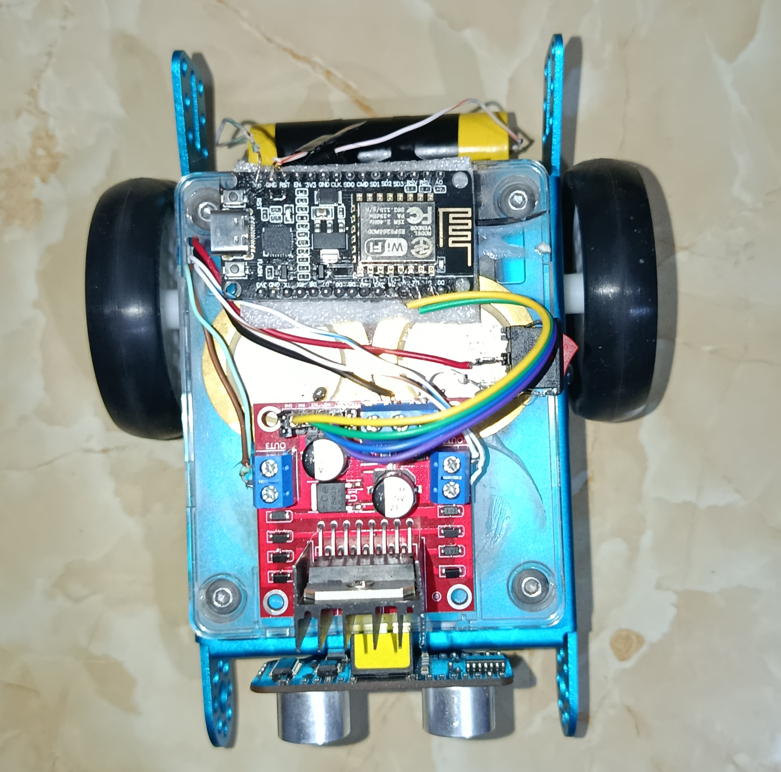
\includegraphics[width=0.45\textwidth]{modelo_vehiculo.png} 
\caption{Vehículo finalizado exhibiendo la tracción diferencial frontal y la rueda loca estabilizadora en la sección posterior.}
\label{fig:vehiculo}
\end{figure}

\section{Discusión y Conclusiones}
Los proyectos de este tipo suelen presentar fallas por problemas de energía o latencia \cite{makerscience}. La estrategia de usar baterías separadas para los motores (potencia) y para el microcontrolador (lógica) fue la solución ideal para mantener el circuito estable. 

Además, se demostró computacionalmente que al ordenar el código para no saturar la pantalla OLED, el procesador se libera y permite un envío de datos constante, logrando una respuesta en tiempo real y tolerante a fallos.

A partir del desarrollo del presente proyecto, se establecen las siguientes conclusiones principales:
\begin{itemize}
    \item \textbf{Optimización de software y baja latencia:} Evitar que la actualización de la pantalla OLED sature el procesador fue clave para lograr que la comunicación ESP-NOW fuera rápida y resultara en un sistema fluido.
    \item \textbf{Diseño estructural y maniobrabilidad:} El rediseño físico implementando dos llantas de tracción y una rueda loca otorgó libertad de movimiento y facilidad para girar sobre el propio eje, superando a los chasis de cuatro ruedas.
    \item \textbf{Interfaz humano-máquina:} Sustituir el control remoto de botones por un guante gestual hizo que la conducción fuera más intuitiva, demostrando el potencial de los sistemas MEMS en la robótica de consumo.
    \item \textbf{Gestión energética y estabilidad:} Separar la alimentación de los motores de la del microcontrolador ESP8266 fue fundamental para aislar el ruido eléctrico y evitar apagones o reinicios esporádicos.
    \item \textbf{Integración de sistemas y seguridad:} El desarrollo de una rutina Failsafe asíncrona garantizó que, ante la pérdida eventual de paquetes de red, el vehículo respondiera de forma segura deteniendo su avance.
\end{itemize}

\section{Actividades Complementarias}
\begin{figure}[htbp]
\centering
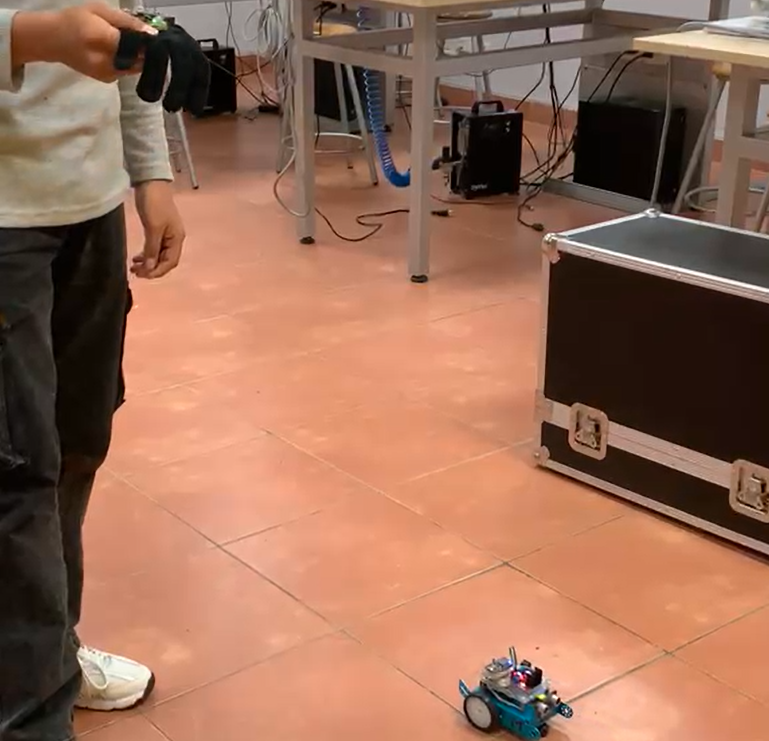
\includegraphics[width=0.4\textwidth]{campo.png} 
\caption{Captura de presentación de prácticas de campo.}
\end{figure}

\begin{figure}[htbp]
\centering
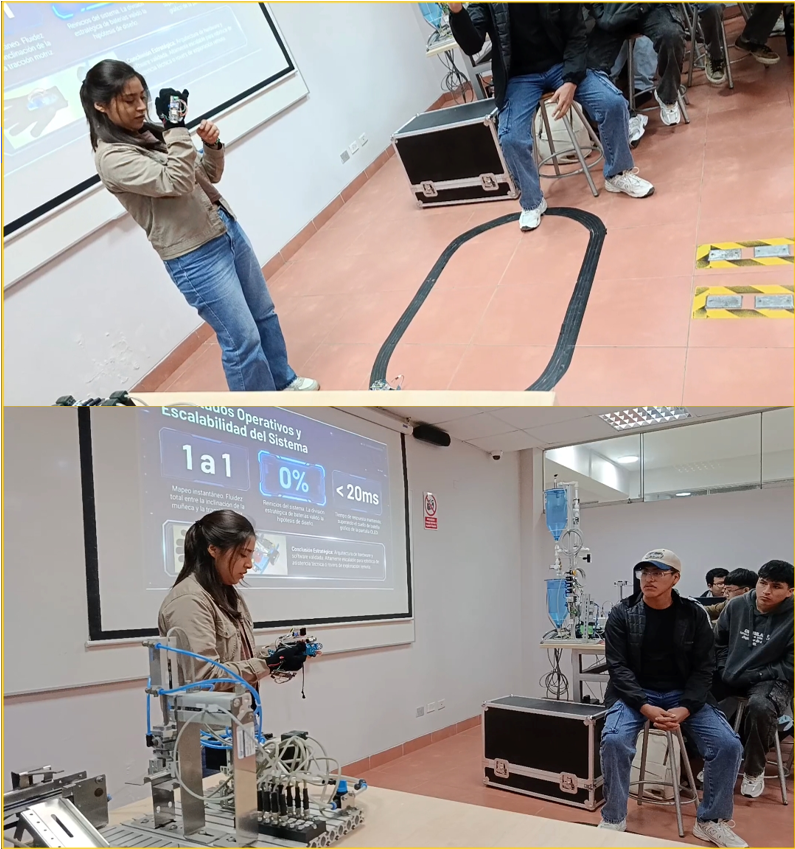
\includegraphics[width=0.4\textwidth]{debate.png} 
\caption{Evidencia de participación en debates/exposición.}
\end{figure}

\begin{thebibliography}{9}
% Referencias en formato APA 7ma edición

\bibitem{makerscience} 
Maker Science. (2025, 12 de agosto). \textit{How I made my own Gesture Controlled Car} [Archivo de Video]. YouTube. https://www.youtube.com/watch?v=VZoVGXVw670

\bibitem{espnow_paper} 
Kuzmanov, I., \& Pasic, R. (2022). ESP-NOW communication protocol with ESP32/ESP8266. \textit{International Scientific Conference Unitech}, 1(1), 145-150. https://www.researchgate.net/publication/362879554

\bibitem{mpu_paper}
Pinto, S. S., \& Singh, A. (2024). Hand gesture recognition robot using IoT techniques and MPU6050. \textit{TIJER - International Research Journal}, 11(5), 132-137. https://tijer.org/tijer/papers/TIJER2405132.pdf

\end{thebibliography}

\section*{Anexos}
El código fuente modificado, que incluye los algoritmos anti-latencia para la gestión I2C de la pantalla OLED y la implementación de la rutina Failsafe en el receptor, se encuentra documentado públicamente en el repositorio oficial del proyecto:
\url{https://github.com/AxelC2code/gesture-sheep-Cart}

\end{document}